\documentclass[t,usenames,dvipsnames]{beamer}
\usetheme{Copenhagen}
\usepackage{amsmath, tikz, xcolor, array}
\setbeamertemplate{headline}{} % remove toc from headers

\title{Polar Form of Complex Numbers}
\author{}
\date{}

\AtBeginSection[]
{
  \begin{frame}
    \frametitle{Table of Contents}
    \tableofcontents[currentsection]
  \end{frame}
}
\DeclareMathOperator\cis{cis}

\begin{document}

\begin{frame}
    \titlepage
\end{frame}

\section{Plot Numbers in the Complex Plane}

\begin{frame}{The Complex Plane}
    The complex plane is very similar to the Cartesian $(x,y)$ plane from algebra. \newline\\
    
    The point $(x,y)$ in the Cartesian plane is represented by \alert{\[z = x + yi\]} in the complex plane.  \newline\\
    
    $x$ is called the \emph{real part} and $y$ is called the \emph{imaginary part}.
\end{frame}

\begin{frame}{The Complex Plane}
    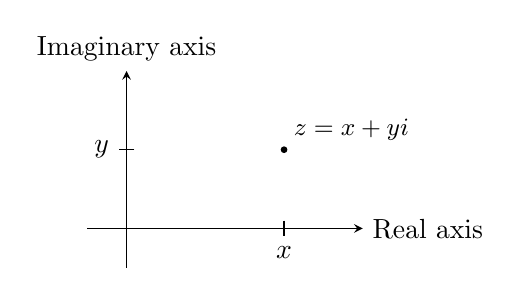
\begin{tikzpicture}
    \draw [->, >=stealth] (-0.5,0) -- (3,0) node [right] {Real axis};
    \draw [->, >=stealth] (0,-0.5) -- (0,2) node [above] {Imaginary axis};
    \draw (2,0.1) -- (2,-0.1) node [below] {$x$};
    \draw (0.1,1) -- (-0.1,1) node [left] {$y$};
    \coordinate (Z) at (2,1);
    \draw [fill=black] (Z) circle (1pt) node [above right] {\small $z=x+yi$};
    \end{tikzpicture}
\end{frame}

\section{Find the Modulus and Argument of a Complex Number}

\begin{frame}{Modulus of a Complex Number}
    The \alert{modulus} of a complex number is the absolute value of it:
    \[
    |z| = |x + yi| = \sqrt{x^2+y^2}
    \]
    and it denotes the \emph{distance} the point is to the origin.
\end{frame}

\begin{frame}{Argument of a Complex Number}
    If we connect out point to the origin, it models an angle drawn in standard position. \newline\\
    
    \begin{center}
    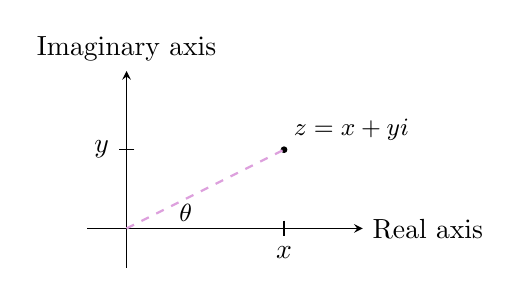
\begin{tikzpicture}
    \draw [->, >=stealth] (-0.5,0) -- (3,0) node [right] {Real axis};
    \draw [->, >=stealth] (0,-0.5) -- (0,2) node [above] {Imaginary axis};
    \draw (2,0.1) -- (2,-0.1) node [below] {$x$};
    \draw (0.1,1) -- (-0.1,1) node [left] {$y$};
    \coordinate (Z) at (2,1);
    \draw [fill=black] (Z) circle (1pt) node [above right] {\small $z=x+yi$};
    \draw [thick, dashed, Plum] (0,0)  -- (Z);
    \node at (0,0) [xshift=0.75cm, yshift=0.2cm] {\small $\theta$};
    \end{tikzpicture}
    \end{center}
\end{frame}

\begin{frame}{Argument of a Complex Number}
    If $z$ is in polar form, the total angle rotated $\theta$ is the \alert{argument} of $z$. \newline\\
    
    The set of all arguments of $z$ is denoted \alert{arg($z$)}. (These can be found by using co-terminal angles).    \newline\\
    
    If $z \neq 0$ and $-\pi < \theta \leq \pi$, then $\theta$ is the \alert{principal argument} of $z$, and is written \alert{$\theta = \text{Arg}(z)$}    \newline\\
    
    We can get the angle rotated via reference angles using
    \[
    \theta ' = \tan^{-1} \left( \frac{y}{x} \right)
    \]
\end{frame}

\begin{frame}{Example 1a.}
    Plot each complex number, find its modulus, real and imaginary parts, arg($z$) and Arg($z$). \newline\\
    
    (a) \quad   $z = \sqrt{3} - i$  \newline\\
    \pause
    The real part of $z$ is $\sqrt{3}$ and the imaginary part of $z$ is $-1$.
\end{frame}

\begin{frame}{Example 1a.}
    \begin{center}
    \begin{tikzpicture}
    \draw [->, >=stealth] (-0.5,0) -- (2,0) node [right] {\small $x$};
    \draw [->, >=stealth] (0,0.5) -- (0,-1.25) node [below] {\small $-yi$};
    \draw [fill=black] (1.5,-0.75) circle (1pt) node [below right] {\small $z=\sqrt{3}-i$};
    \draw (1.5,0.1) -- (1.5,-0.1) node [above, yshift=0.2cm] {\tiny $\sqrt{3}$};
    \draw (0.1,-0.75) -- (-0.1,-0.75) node [left] {\tiny $-1$};
    \end{tikzpicture}
    \end{center}
\pause
The modulus is
\[
|z| = \sqrt{(\sqrt{3})^2 + (-1)^2} = \sqrt{4} = 2
\]
\end{frame}

\begin{frame}{Example 1a.}
\emph{Tip:} Find the principal argument of $z$, denoted Arg($z$), before finding the general solution, arg($z$).
\pause
    \begin{center}
    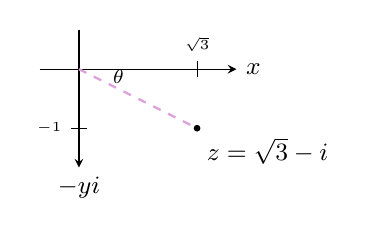
\begin{tikzpicture}
    \draw [->, >=stealth] (-0.5,0) -- (2,0) node [right] {\small $x$};
    \draw [->, >=stealth] (0,0.5) -- (0,-1.25) node [below] {\small $-yi$};
    \draw [fill=black] (1.5,-0.75) circle (1pt) node [below right] {\small $z=\sqrt{3}-i$};
    \draw (1.5,0.1) -- (1.5,-0.1) node [above, yshift=0.2cm] {\tiny $\sqrt{3}$};
    \draw (0.1,-0.75) -- (-0.1,-0.75) node [left] {\tiny $-1$};
    \draw [thick, dashed, Plum] (0,0) -- (1.5,-0.75);
    \node at (0,0) [xshift=0.5cm, yshift=-0.1cm] {\scriptsize $\theta$};
    \end{tikzpicture}
    \end{center}    
    \pause
    \[
    \text{Arg}(z) = \tan^{-1}\left( \frac{-1}{\sqrt{3}}\right) = -30^\circ = -\frac{\pi}{6}
    \]
\end{frame}

\begin{frame}{Example 1a.}
    To find arg($z$), use co-terminal angles with the answer you got for Arg($z$) to get
    \[
    \text{arg}(z) = -\frac{\pi}{6} + 2\pi k
    \]
    where $k$ is an integer.
\end{frame}

\begin{frame}{Example 1b.}
    (b) \quad   $z = -2+4i$  \newline\\
    \pause
    The real part of $z$ is $-2$ and the imaginary part of $z$ is $4$.
\end{frame}

\begin{frame}{Example 1b.}
    \begin{center}
    \begin{tikzpicture}
    \draw [->, >=stealth] (0.5,0) -- (-2,0);
    \draw [->, >=stealth] (0,-0.5) -- (0,2.5);
    \coordinate (Z) at (-1,2);
    \draw [fill=black] (Z) circle (1pt) node [above left] {$z = -2+4i$};
    \draw (-1,0.1) -- (-1,-0.1) node [below] {\scriptsize $-2$};
    \draw (-0.1,2) -- (0.1,2) node [right] {\scriptsize $4$};
    \end{tikzpicture}
    \end{center}
\pause
The modulus is
\[
|z| = \sqrt{(-2)^2 + 4^2} = \sqrt{20} = 2\sqrt{5}
\]
\end{frame}


\begin{frame}{Example 1b.}
    Arg($z$) is
    \[
    \tan^{-1} \left(\frac{4}{-2}\right) = \tan^{-1}(-2) \approx -63.4^\circ
    \]
\pause
Since $z$ is in the 2nd quadrant, we can put a $63.4^\circ$ reference angle (\emph{Reminder}: $63.4^\circ \approx \tan^{-1}(2)$) in quadrant II, so the total angle rotated is about $116.6^\circ$, or $\pi - \tan^{-1}(2)$ to be exact.   \newline\\      \pause
Thus, Arg($z$) = $\pi - \tan^{-1}(2)$, \newline\\
\pause  and \newline\\
arg($z$) = $\left(\pi - \tan^{-1}(2)\right) + 2\pi k$
\end{frame}

\begin{frame}{Example 1c.}
    (c) \quad   $z = 3i$  \newline\\
    \pause
    The real part of $z$ is 0 and the imaginary part of $z$ is $3$.
\end{frame}

\begin{frame}{Example 1c.}
\begin{center}
    \begin{tikzpicture}
    \draw [->, >=stealth] (-0.5,0) -- (2,0);
    \draw [->, >=stealth] (0,-0.5) -- (0,2);
    \draw (0.1,1.5) -- (-0.1,1.5) node [left] {\scriptsize 3};
    \draw [fill=black] (0,1.5) circle (1.5pt) node [right] {\scriptsize $z = 3i$};
    \end{tikzpicture}
\newline\\
\pause
The modulus is 3.   \newline\\
\pause 
Arg($z$) = $\frac{\pi}{2}$  \newline\\
\pause
arg($z$) = $\frac{\pi}{2} + 2\pi k$
\end{center}
\end{frame}

\begin{frame}{Example 1d.}
   (d) \quad   $z = -117$  \newline\\
    \pause
    The real part of $z$ is $-117$ and the imaginary part of $z$ is 0.
\end{frame}

\begin{frame}{Example 1d.}
\begin{center}
    \begin{tikzpicture}
    \draw [<->, >=stealth] (-2,0) -- (2,0);
    \draw [->, >=stealth] (0,0) -- (0,1);
    \draw (-1.5,0.1) -- (-1.5,-0.1) node [below] {\scriptsize $-117$};
    \draw [fill=black] (-1.5,0) circle (1.5pt) node [above] {\scriptsize $z=-117$};
    \end{tikzpicture}
\newline\\  \pause
The modulus of $z$ is 117.  \newline\\  \pause
Arg($z$) = $\pi$    \newline\\      \pause
arg($z$) = $\pi + 2\pi k$
\end{center}
\end{frame}

\section{Write Complex Numbers in Polar Form and Vice Versa}

\begin{frame}{Write Complex Numbers in Polar Form}
    Writing polar form of complex numbers is a lot like writing rectangular coordinates as polar coordinates.   \newline\\
    \begin{center}
    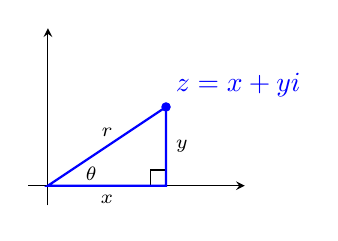
\begin{tikzpicture}
    \draw [->, >=stealth] (-0.25,0) -- (2.5,0);
    \draw [->, >=stealth] (0,-0.25) -- (0,2);
    \draw (1.5,0) rectangle +(-0.2,0.2);
    \draw [thick, color=blue] (0,0) -- (1.5,0) -- (1.5,1) -- cycle;
    \node at (0.75,0) [below] {\scriptsize $x$};
    \node at (1.5,0.5) [right] {\scriptsize $y$};
    \node at (0.75,0.5) [above] {\scriptsize $r$};
    \draw [color=blue, fill=blue] (1.5,1) circle (1.5pt) node [above right] {$z = x+yi$};
    \node at (0.55,0.15) {\scriptsize $\theta$};
    \end{tikzpicture}
    \end{center}
\pause
Using the fact that $x = r\cos\theta$ and $y = r\sin\theta$, we get
\begin{align*}
    \onslide<2->{z &= x + yi\\[8pt]}
    \onslide<3->{&= r\cos\theta + (r\sin\theta)i \\[8pt]}
    \onslide<4->{&=r(\cos\theta + i\sin\theta)}
\end{align*}
\end{frame}

\begin{frame}{Write Complex Numbers in Polar Form}
    $r(\cos\theta + i\sin\theta)$ is often abbreviated $r\cis\theta$.
\end{frame}

\begin{frame}{Example 2a.}
    Write each in polar form.   \newline\\
    (a) \quad $z = \sqrt{3} - i$    \newline\\  \pause
    From Example 1a, $r = 2$, and $\theta = -\frac{\pi}{6}$.    \newline\\  
    Thus, $z = 2\cis\left(-\frac{\pi}{6}\right)$
\end{frame}

\begin{frame}{Example 2b.}
    Write each in polar form.   \newline\\
    (b) \quad $z = -2 + 4i$    \newline\\  \pause
    From Example 1b, $r = 2\sqrt{5}$, and $\theta = \pi - \tan^{-1}(2)$.    \newline\\  
    Thus, $z = \left(2\sqrt{5}\right)\cis\left(\pi - \tan^{-1}(2)\right)$
\end{frame}

\begin{frame}{Example 2c.}
    Write each in polar form.   \newline\\
    (c) \quad $z = 3i$    \newline\\  \pause
    From Example 1c, $r = 3$, and $\theta = \frac{\pi}{2}$.    \newline\\  
    Thus, $z = 3\cis\left(\frac{\pi}{2}\right)$
\end{frame}

\begin{frame}{Example 2d.}
    Write each in polar form.   \newline\\
    (d) \quad $z = -117$    \newline\\  \pause
    From Example 1d, $r = 117$, and $\theta = \pi$.    \newline\\  
    Thus, $z = 117\cis\left(\pi\right)$
\end{frame}

\begin{frame}{Write Complex Polar Numbers in Rectangular Form}
    Going backwards, expand and evaluate $\cis$ and distribute the modulus $r$.
\end{frame}

\begin{frame}{Example 3a.}
    Write each of the following in rectangular form. \newline\\
    (a) \quad   $4\cis\left(\frac{2\pi}{3}\right)$  \newline\\
    \begin{align*}
        \onslide<2->{4\cis\left(\frac{2\pi}{3}\right) &= 4\left(\cos\left(\frac{2\pi}{3}\right) + i\sin\left(\frac{2\pi}{3}\right)\right)}    \\[8pt]
        \onslide<3->{&=4\left(-\frac{1}{2} + \frac{\sqrt{3}}{2}i\right)}  \\[8pt]
        \onslide<4->{&= -2+2i\sqrt{3}}
    \end{align*}
\end{frame}

\begin{frame}{Example 3b.}
    (b) \quad   $2\cis\left(-\frac{3\pi}{4}\right)$ \newline\\
    \begin{align*}
        \onslide<2->{2\cis\left(-\frac{3\pi}{4}\right) &= 2\left(\cos\left(-\frac{3\pi}{4}\right) + i\sin\left(-\frac{3\pi}{4}\right)\right)}   \\[8pt]
        \onslide<3->{&= 2\left(-\frac{\sqrt{2}}{2} - \frac{\sqrt{2}}{2}i \right)}    \\[8pt]
        \onslide<4->{&= -\sqrt{2}-i\sqrt{2}}
    \end{align*}
\end{frame}

\begin{frame}{Example 3c.}
    (c) \quad   $3\cis(0)$  \newline\\
    \begin{align*}
        \onslide<2->{3\cis(0) &= 3(\cos(0) + i\sin(0))} \\[8pt]
        \onslide<3->{&= 3(1 + 0) = 3}
    \end{align*}
\end{frame}

\begin{frame}{Example 3d.}
    (d) \quad $\cis\left(\frac{\pi}{2}\right)$  \newline\\
    \begin{align*}
        \onslide<2->{\cis\left(\frac{\pi}{2}\right) &= \cos\left(\frac{\pi}{2}\right) + i\sin\left(\frac{\pi}{2}\right)}    \\[8pt]
        \onslide<3->{&= 0 + 1i = i}
    \end{align*}
\end{frame}


\section{Perform Arithmetic Operations on Complex Numbers in Polar Form}

\begin{frame}{Arithmetic Operations on Complex Numbers in Polar Form}
The rules for multiplying, dividing, and finding powers of complex numbers are the same as those for exponents.    \newline\\
\pause 

\setlength{\extrarowheight}{10pt}
\begin{tabular}{ccc}
    \textbf{Rule} & \textbf{Exponents} & \textbf{Complex Numbers}    \\ \hline
    Product & $3x^{15}\cdot 4x^7 = 12x^{22}$ & $3\cis15^\circ \cdot 4 \cis 7^\circ = 12 \cis 22^\circ$ \\[10pt]
    Quotient & $\dfrac{3x^{15}}{4x^7} = \dfrac{3}{4}x^8$ &
    $\dfrac{3\cis15^\circ}{4\cis7^\circ} = \dfrac{3}{4}\cis 8^\circ$ \\[10pt] 
    Power & $(3x^{15})^2 = 9x^{30}$ & $(3\cis15^\circ)^2 = 9\cis30^\circ$ \\[15pt]
\end{tabular}

The Power Rule is known as DeMoivre's Theorem
\end{frame}

\begin{frame}{Example 4a}
    Let $z=2\sqrt{3}+2i$ and $w=-1+i\sqrt{3}$. Find each of the following and write your answers in rectangular form.    \newline\\
    (a) \quad $zw$  \newline\\
    \pause
    In polar form, $z=4\cis\dfrac{\pi}{6}$ and $w=2\cis\dfrac{2\pi}{3}$.   \\[15pt]  \pause
    Thus, $zw = \left(4\cis\dfrac{\pi}{6}\right)\left(2\cis\dfrac{2\pi}{3}\right)=8\cis\dfrac{5\pi}{6}$   \\[15pt]  \pause
    In rectangular form, $8\cis\dfrac{5\pi}{6} = -4\sqrt{3} + 4i$
\end{frame}

\begin{frame}{Example 4b}
    (b) \quad $w^5$ \newline\\
    \pause
    $w^5 = \left(2\cis\dfrac{2\pi}{3}\right)^5 = 32\cis\dfrac{10\pi}{3}$  \\[15pt]   \pause
    $32\cis\dfrac{10\pi}{3} = 32\cis\dfrac{4\pi}{3}=-16-16i\sqrt{3}$
\end{frame}

\begin{frame}{Example 4c}
(c) \quad $\dfrac{z}{w}$    \newline\\  \pause
\begin{align*}
    \onslide<2->{\dfrac{z}{w} &= \dfrac{4\cis\frac{\pi}{6}}{2\cis\frac{2\pi}{3}}} \\[15pt]
    \onslide<3->{&= 2\cis\left(\frac{\pi}{6}-\frac{2\pi}{3}\right)} \\[15pt]
    \onslide<4->{&=2\cis\left(-\frac{\pi}{2}\right)=-2i}
\end{align*}
\end{frame}

\section{Find Roots of Complex Numbers}

\begin{frame}{Find Roots of Complex Numbers}
    Recall that $\sqrt[n]{x} = x^{1/n}$.   \newline\\
    We can reverse DeMoivre's Theorem to get roots of complex numbers.    \newline\\  \pause
    Given $w$ and $z$ are complex numbers, if there is a natural number $n$ such that $w^n = z$, then $w$ is an $n$th root of $z$.
\end{frame}

\begin{frame}{Find Roots of Complex Numbers}
    Let $z \neq 0$ be a complex numbrer with polar form $z=r\cis\theta$. For each natural number $n$, $z$ has $n$ distinct $n$th roots (denoted by $w_0, w_1, \dots, w_{n-1}$, given by
    \[
    w_k = \sqrt[n]{r}\cis\left(\dfrac{\theta + 2\pi k}{n}\right)
    \]
    \pause
    \emph{Tip:} You can still work in degrees and convert your answers to radians.
\end{frame}

\begin{frame}{Example 5a}
    Find each of the following. \newline\\
    (a) \quad both square roots of $z = -2 + 2i\sqrt{3}$    \pause
    \begin{align*}
        \onslide<2->{z &= 4\cis\dfrac{2\pi}{3} \left(\text{or } 4\cis120^\circ\right)} \\
        \onslide<3->{&=4^{1/2}\left(\cos\frac{120^\circ+360k}{2}+i\sin\frac{120^\circ+360k}{2}\right)}  \\
        \onslide<4->{&=2\left(\cos\left(60^\circ+180k\right) + i\sin\left(60^\circ+180k\right)\right)} \\
        \onslide<5->{&=2\cis60^\circ, 2\cis240^\circ} \\
        \onslide<6->{&=1+i\sqrt{3}, \quad -2+2i\sqrt{3}}
    \end{align*}
\end{frame}

\begin{frame}{Example 5b}
    (b) \quad the four fourth roots of $z=-16$ \pause
    \begin{align*}
        \onslide<2->{z &= 16\cis180^\circ} \\
        \onslide<3->{&=16^{1/4}\cis\left(\frac{180^\circ+360k}{4}\right)} \\
        \onslide<4->{&=2\cis\left(45^\circ+90k\right)}   \\
    \end{align*}
    \onslide<5->{$2\cis45^\circ, 2\cis135^\circ, 2\cis225^\circ, 2\cis315^\circ$} \newline\\
    \onslide<6->{$\sqrt{2}+i\sqrt{2}, -\sqrt{2}+i\sqrt{2}, -\sqrt{2}-i\sqrt{2}, \sqrt{2}-i\sqrt{2}$}
\end{frame}

\begin{frame}{Visualization of Solutions}
    \begin{center}
    \begin{tikzpicture}
    \draw [<->, >=stealth] (-3.5,0) -- (3.5,0) node [right] {$x$};
    \draw [<->, >=stealth] (0,-3.5) -- (0,3.5) node [right] {$yi$};
    \foreach \x in {-3,-2,-1,,,1,2,3}
    \draw (\x,0.1) -- (\x,-0.1) node [below] {\scriptsize $\x$};
    \foreach \y in {-3,-2,-1,,,1,2,3}
    \draw (0.1,\y) -- (-0.1,\y) node [left] {\scriptsize $\y i$};
    \coordinate (A) at (1.414,1.414);
    \coordinate (B) at (-1.414,1.414);
    \coordinate (C) at (-1.414,-1.414);
    \coordinate (D) at (1.414,-1.414);
    \draw [color=red, fill = red] (A) circle (1.5pt);
    \draw [color=red, fill = red] (B) circle (1.5pt);
    \draw [color=red, fill = red] (C) circle (1.5pt);
    \draw [color=red, fill = red] (D) circle (1.5pt);
    \draw [color=red, dashed] (A) -- (B) -- (C) -- (D) -- cycle;
    \end{tikzpicture}
    \end{center}
\end{frame}

\begin{frame}{Example 5c}
    (c) \quad the three cube roots of $z = \sqrt{2} + i\sqrt{2}$ \pause
    \begin{align*}
        \onslide<2->{z &= 2\cis\left(45^\circ\right)} \\
        \onslide<3->{&= 2^{1/3}\left(\cis\left(\frac{45^\circ + 360k}{3}\right)\right)} \\
        \onslide<4->{&= \sqrt[3]{2}\cis\left(15^\circ + 120k\right)} \\
    \end{align*}
    \onslide<5->{$\sqrt[3]{2}\cis15^\circ, \sqrt[3]{2}\cis135^\circ, \sqrt[3]{2}\cis255^\circ$}  \newline\\
\end{frame}

\begin{frame}{Example 5d}
    (d) \quad the five fifth roots of $z = 1$   \pause
    \begin{align*}
        \onslide<2->{z &= 1\cis0} \\
        \onslide<3->{&= \cis\left(\frac{0+360k}{5}\right)} \\
        \onslide<4->{&=\cis\left(0+72k\right)} \\
    \end{align*}
    \onslide<5->{$1$, $\cis72^\circ$, $\cis144^\circ$, $\cis216^\circ$, $\cis288^\circ$}
\end{frame}
\end{document}
